% Book pp. 75-77 (PDF pp. 76-78)
\section{Solving Quadratic Inequalities}

In year one we learnt about quadratic functions, how to solve them algebraically
and how to illustrate them graphically. Remember that quadratic functions are of
the form

$M(x) = ax^2 + bx + c$, where $a, b, c \in R$, $a \ne 0$.

Combining this knowledge and what we know about linear inequalities, we can
represent general quadratic inequalities in the forms;
\begin{enumerate}
  \item $ax^2 + bx + c < w$
  \item $ax^2 + bx + c > w$
  \item $ax^2 + bx + c \le w$
  \item $ax^2 + bx + c \ge w$, where $w$ is a constant.
\end{enumerate}
To find the solution to a quadratic inequality of any of the forms above:
\begin{enumerate}
  \item First determine the value of $w$
  \item Simplify the inequality so that one side is zero
  \item Factorise to determine the range of values for $x$
  \item Represent it graphically to know the solution region
\end{enumerate}

\begin{activity}{Activity 2.6 -- Individual/Group Exploration of Quadratic Inequalities}
\begin{enumerate}
  \item Brainstorm how you would solve the inequalities:
  \item $x^2 - 3x - 10 > 0$ and $-2x^2 + 5x \le 3$.
  \item Discuss multiple approaches (factorising, completing the square or using
  the quadratic formula).
  \item Consider when the expression is equal to zero and how this can help
  determine the solution.
  \item Draw separately the graph of each of the quadratic inequalities to
  understand the regions where the inequality is true or false.
  \item Share your observations from the process with a peer.
\end{enumerate}
\end{activity}

\begin{example}{Example 2.18}
Find the solution to the inequality $x^2 - 2x - 15 < 0$.

\solution
\textbf{Step 1:} Factorise the left-hand side of the inequality

$x^2 - 2x - 15 = (x + 3)(x - 5)$

Hence $(x + 3)(x - 5) < 0$

\textbf{Step 2:} Find the critical values

$x = 5$ and $x = -3$

\textbf{Step 3:}

\textbf{Method 1:} Represent the extreme values of the expected solution on a number
line and test them.
\begin{center}
\begin{tikzpicture}[x=1.1cm]
  \draw[{Stealth}-{Stealth}] (-4.8,0) -- (6.8,0);
  \foreach \x in {-4,...,6} {
    \draw (\x,0.08) -- (\x,-0.08);
    \node[below, font=\tiny] at (\x,-0.05) {$\x$};
  }
  \draw[green!60!black, thick, {Stealth}-] (-4.7,0.45) -- (-3,0.45);
  \node[green!60!black, font=\scriptsize, above] at (-3.9,0.5) {$x < -3$};
  \draw[orange!80!black, thick] (-3,0.45) -- (5,0.45);
  \node[orange!80!black, font=\scriptsize, above] at (1,0.5) {$-3 < x < 5$};
  \draw[blue, thick, -{Stealth}] (5,0.45) -- (6.7,0.45);
  \node[blue, font=\scriptsize, above] at (5.9,0.5) {$x > 5$};
  \foreach \x in {-3,5} {
    \fill[white] (\x,0.45) circle (2.2pt);
    \draw (\x,0.45) circle (2.2pt);
  }
\end{tikzpicture}
\end{center}
\figcaption{2.7}{Representing possible solutions to quadratic inequalities on number lines}

\begin{center}
\small\setlength{\tabcolsep}{4pt}
\begin{tabular}{|p{2.7cm}|p{1.4cm}|c|c|c|l|}
\hline
\textbf{Possible Solution Regions} & \textbf{Test Values} & $\boldsymbol{x + 3}$ &
$\boldsymbol{x - 5}$ & $\boldsymbol{(x + 3)(x - 5)}$ & \textbf{Sign} \\
\hline
$x < -3$ & $-4$ & $-1$ & $-9$ & 9 & Positive \\
\hline
$-3 < x < 5$ & 3 & 6 & $-2$ & $-12$ & Negative \\
\hline
$x > 5$ & 6 & 9 & 1 & 9 & Positive \\
\hline
\end{tabular}
\end{center}

\textbf{Step 4:} Select the solution region that corresponds to the sign satisfying the
inequality.

Since $x^2 - 2x - 15 < 0$ holds for only values of $x$ for which the product of the
factors is negative (less than zero), $-3 < x < 5$ is the solution to the inequality.

\textbf{OR}

\textbf{Step 3:}

\textbf{Method 2:} Graph the quadratic inequality
\begin{center}
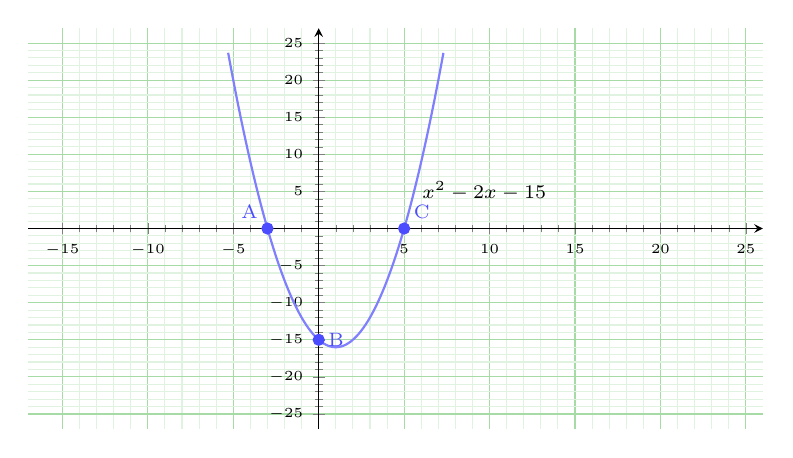
\begin{tikzpicture}
\begin{axis}[
  width=0.9\linewidth, height=0.55\linewidth,
  axis lines=middle, grid=both, minor tick num=4,
  grid style={green!60!black!35}, minor grid style={green!60!black!12},
  xmin=-17, xmax=26, ymin=-27, ymax=27,
  xtick={-15,-10,...,25}, ytick={-25,-20,...,25},
  tick label style={font=\tiny}
]
\addplot[blue!50, thick, domain=-5.3:7.3, samples=100] {x^2 - 2*x - 15};
\addplot[only marks, mark=*, blue!70] coordinates {(-3,0) (5,0) (0,-15)};
\node[blue!70, above left, font=\scriptsize] at (axis cs:-3,0) {A};
\node[blue!70, above right, font=\scriptsize] at (axis cs:5,0) {C};
\node[blue!70, right, font=\scriptsize] at (axis cs:0,-15) {B};
\node[right, font=\scriptsize] at (axis cs:5.5,5) {$x^2 - 2x - 15$};
\end{axis}
\end{tikzpicture}
\end{center}
\figcaption{2.8}{Quadratic graph of $x^2 - 2x - 15$}

\textbf{Step 4:} Identify the portion of the graph that satisfies the inequality. In this
case, the portion below the x-axis.
\begin{center}
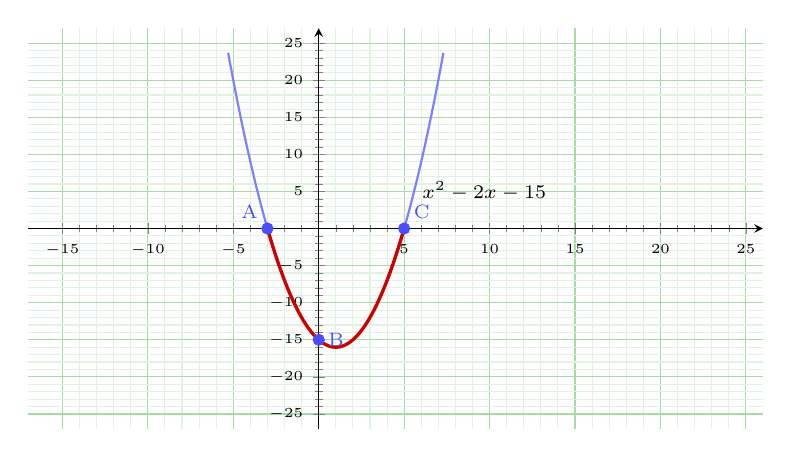
\begin{tikzpicture}
\begin{axis}[
  width=0.9\linewidth, height=0.55\linewidth,
  axis lines=middle, grid=both, minor tick num=4,
  grid style={green!60!black!35}, minor grid style={green!60!black!12},
  xmin=-17, xmax=26, ymin=-27, ymax=27,
  xtick={-15,-10,...,25}, ytick={-25,-20,...,25},
  tick label style={font=\tiny}
]
\addplot[blue!50, thick, domain=-5.3:7.3, samples=100] {x^2 - 2*x - 15};
\addplot[red!80!black, very thick, domain=-3:5, samples=60] {x^2 - 2*x - 15};
\addplot[only marks, mark=*, blue!70] coordinates {(-3,0) (5,0) (0,-15)};
\node[blue!70, above left, font=\scriptsize] at (axis cs:-3,0) {A};
\node[blue!70, above right, font=\scriptsize] at (axis cs:5,0) {C};
\node[blue!70, right, font=\scriptsize] at (axis cs:0,-15) {B};
\node[right, font=\scriptsize] at (axis cs:5.5,5) {$x^2 - 2x - 15$};
\end{axis}
\end{tikzpicture}
\end{center}
\figcaption{2.9}{Quadratic graph of $x^2 - 2x - 15$ with solution}

Thus $-3 < x < 5$
\end{example}

% Book pp. 78-79 (PDF pp. 79-80)
\begin{example}{Example 2.19}
Find the solution to the inequality $-5x^2 + 12x - 7 > 0$.

\solution
\textbf{Step 1:} Factorise the left-hand side of the inequality

$-5x^2 + 12x - 7 = (-5x + 7)(x - 1)$

Hence $(-5x + 7)(x - 1) > 0$

\textbf{Step 2:} Find the critical values

$x = \frac{7}{5}$ and $x = 1$.

\textbf{Step 3:} Represent the extreme values of the expected solution on a number line
and test them.
\begin{center}
\begin{tikzpicture}[x=3.6cm]
  \draw[{Stealth}-{Stealth}] (-0.9,0) -- (2.5,0);
  \foreach \x in {-0.8,-0.6,...,2.4} {
    \draw (\x,0.08) -- (\x,-0.08);
    \node[below, font=\tiny] at (\x,-0.05) {\pgfmathprintnumber{\x}};
  }
  \draw[green!60!black, thick, {Stealth}-] (0.55,0.45) -- (1,0.45);
  \node[green!60!black, font=\scriptsize, above] at (0.78,0.5) {$x < 1$};
  \draw[brown!80!black, thick] (1,0.3) -- (1.4,0.3);
  \node[brown!80!black, font=\scriptsize, above] at (1.2,0.55) {$1 < x < 1.4$};
  \draw[blue, thick, -{Stealth}] (1.4,0.45) -- (1.85,0.45);
  \node[blue, font=\scriptsize, above] at (1.62,0.5) {$x > 1.4$};
  \fill[white] (1,0.45) circle (2.2pt); \draw (1,0.45) circle (2.2pt);
  \fill[white] (1.4,0.45) circle (2.2pt); \draw (1.4,0.45) circle (2.2pt);
  \fill[white] (1,0.3) circle (2.2pt); \draw (1,0.3) circle (2.2pt);
  \fill[white] (1.4,0.3) circle (2.2pt); \draw (1.4,0.3) circle (2.2pt);
\end{tikzpicture}
\end{center}
\figcaption{2.10}{Representing quadratic solution on number line 2}

\begin{center}
\small\setlength{\tabcolsep}{4pt}
\begin{tabular}{|p{2.7cm}|p{1.4cm}|c|c|c|l|}
\hline
\textbf{Possible Solution Regions} & \textbf{Test Values} & $\boldsymbol{-5x + 7}$ &
$\boldsymbol{x - 1}$ & $\boldsymbol{(-5x + 7)(x - 1)}$ & \textbf{Sign} \\
\hline
$x < 1$ & 0 & 7 & $-1$ & $-7$ & Negative \\
\hline
$1 < x < 1.4$ & 1.2 & 1 & 0.2 & 0.2 & Positive \\
\hline
$x > 1.4$ & 3 & $-8$ & 2 & $-16$ & Negative \\
\hline
\end{tabular}
\end{center}

\textbf{Step 4:} Select the solution region that corresponds to the sign satisfying the
inequality.

Since $-5x^2 + 12x - 7 > 0$ holds for only values of $x$ for which the product of the
factors is positive (greater than zero), $1 < x < 1.4$ is the solution to the inequality.
\end{example}

\begin{activity}{Activity 2.7 -- Graphical Solution to $-5x^2 + 12x - 7 > 0$}
Represent the solution to $-5x^2 + 12x - 7 > 0$ graphically and share the results
with a classmate.
\end{activity}

\begin{activity}{Activity 2.8 -- Research on Quadratic Inequalities}
\begin{enumerate}
  \item Conduct research on the behaviour of solutions to maximum and
  minimum curves of quadratic functions.
\end{enumerate}
\textbf{Instructions:}
\begin{enumerate}
  \item[a.] Explore the nature of the solution when a quadratic function with a
  minimum curve is:
  \begin{enumerate}
    \item[i.] greater than zero
    \item[ii.] less than zero
  \end{enumerate}
  \item[b.] Explore the nature of the solution when a quadratic function with a
  maximum curve is:
  \begin{enumerate}
    \item[i.] less than zero
    \item[ii.] greater than zero
  \end{enumerate}
  \item[c.] Include graphical representations to support your argument.
  \item[d.] Consult open education resources, YouTube, textbooks, etc.
  \item[e.] Provide references to the sources you consult and use.
\end{enumerate}
\end{activity}
